	\begin{flushleft}
Prueba de Hipótesis sirve para validar aseveraciones sobre la población tomando como evidencia los datos de la muestra.
sean:\\
	
$\pmb{H_O}$: La hipótesis nula.\\
$\pmb{H_A}$: La hipótesis alternativa.\\
$\pmb{\theta}$ : Estimador.\\
$\pmb{\alpha}$: El nivel de significancia.\\

	\end{flushleft}
	\begin{enumerate}
\item	Se definen las hipótesis $H_0$ y $H_A$.\\
		donde $H_0$ asevera que no hay diferencias significativas en la población para poder aseverar $H_A$. Pueden hallarse tres 	diferentes casos:\\


\begin{enumerate}
\begin{minipage}[b]{\textwidth}
    \begin{minipage}[b]{0.3 \textwidth}\item
    	\begin{align*}
    	H_0&: \theta = \theta_0,\\
    	H_A&: \theta \neq \theta_0.
    	\end{align*}
        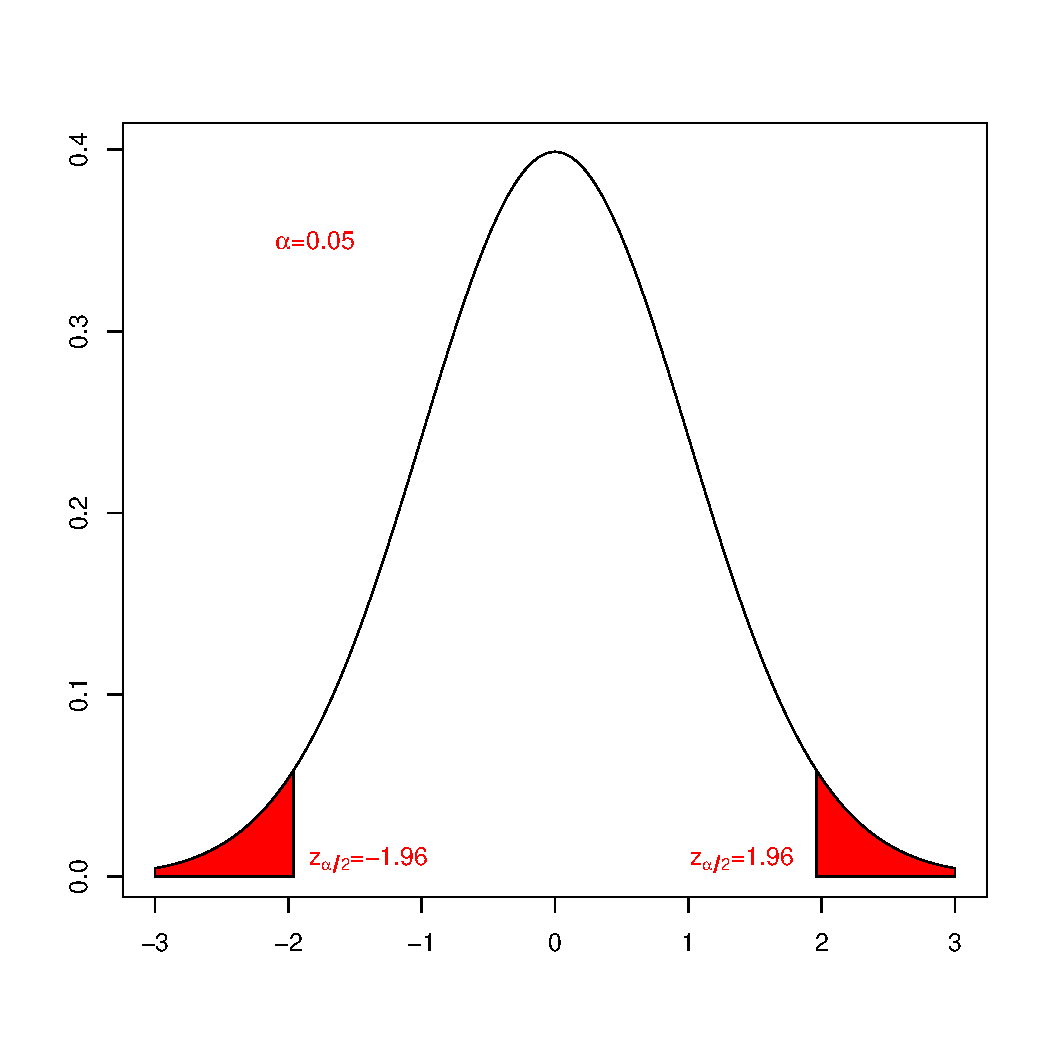
\includegraphics[height=5cm, width=6cm]{z05id.pdf}
    	\end{minipage} \hfill
    \begin{minipage}[b]{0.3 \textwidth}\item
		\begin{align*}
		H_0&: \theta \leq \theta_0,\\
    	H_A&: \theta > \theta_0. 
		\end{align*}
		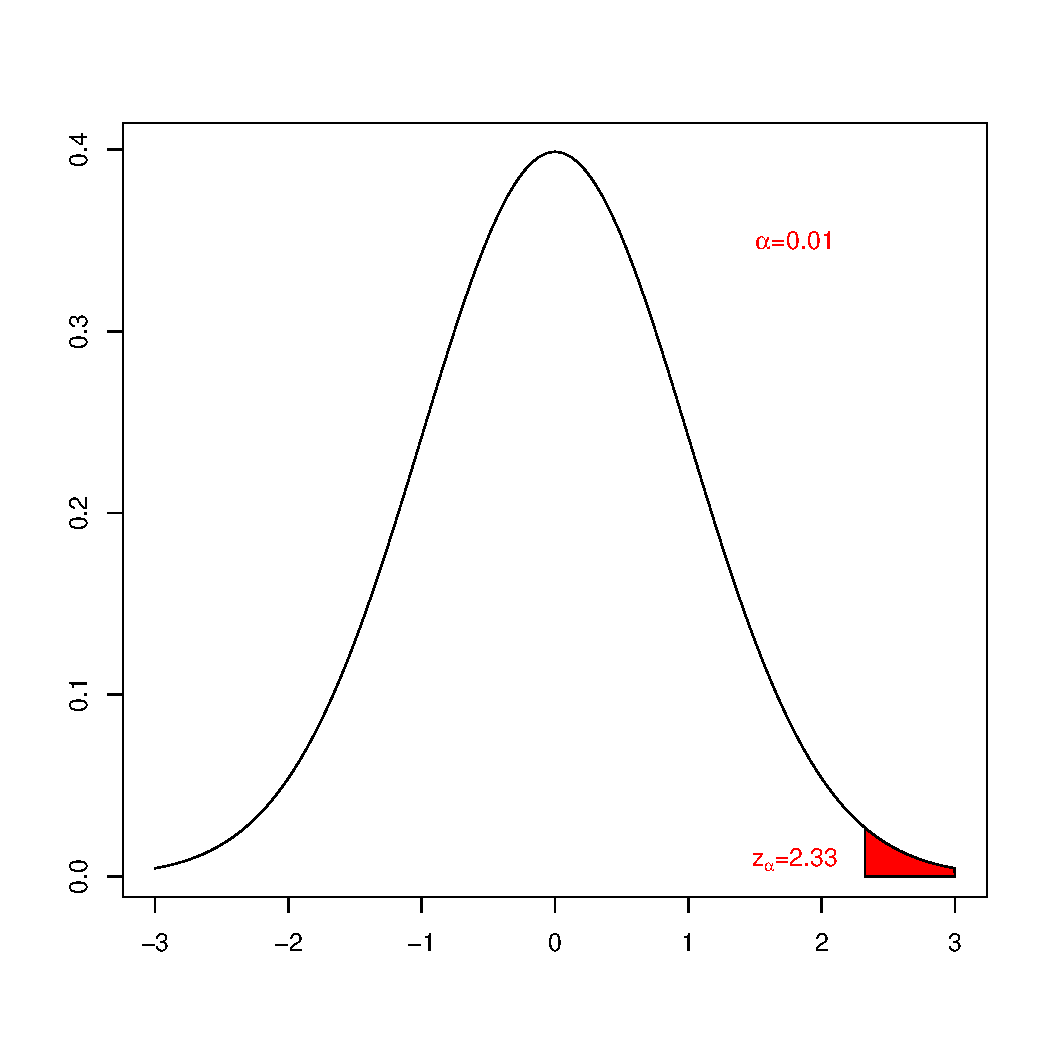
\includegraphics[height=5cm, width=6cm]{z01d.pdf}
		\end{minipage} \hfill
    \begin{minipage}[b]{0.3 \textwidth}\item
		\begin{align*}
		H_0&: \theta \geq \theta_0,\\
    	H_A&: \theta < \theta_0. 
		\end{align*}
		  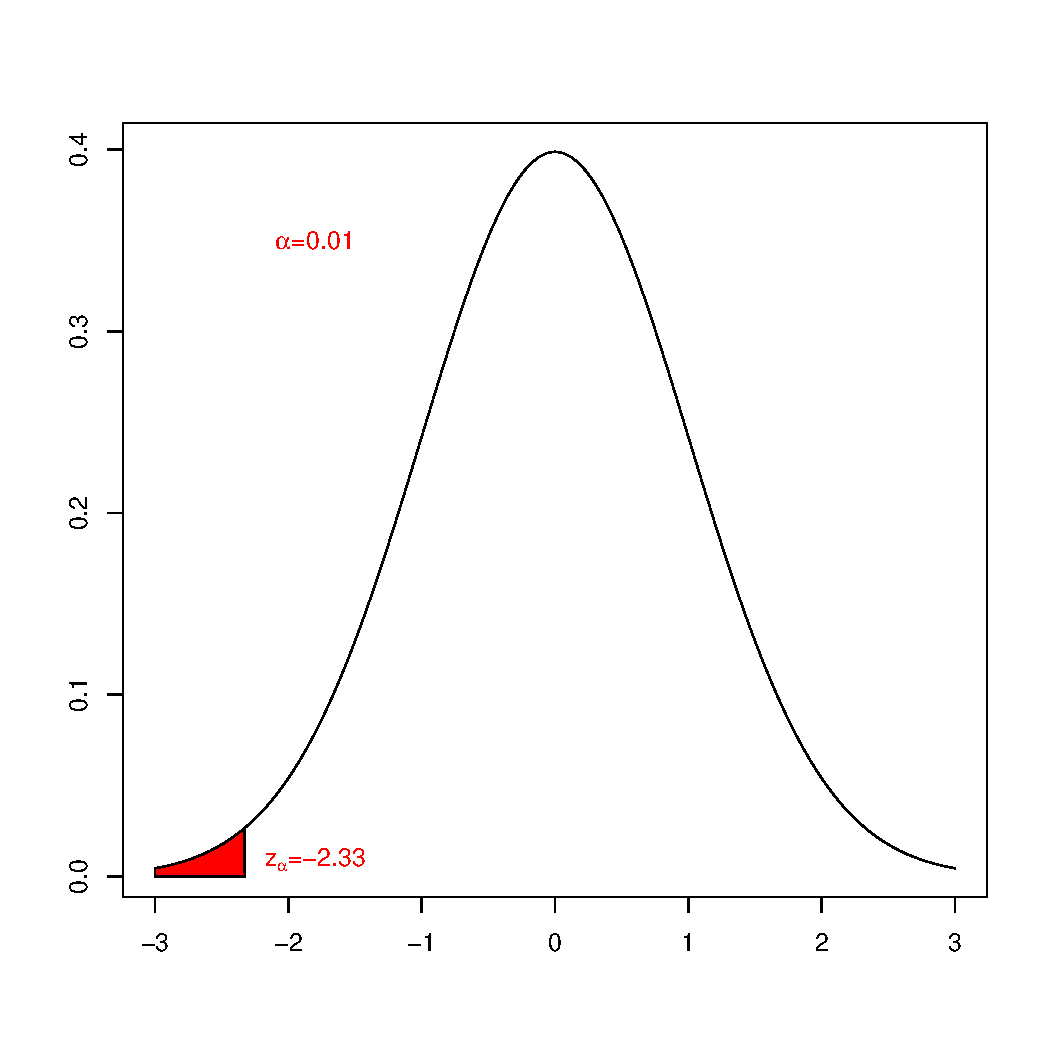
\includegraphics[height=5cm, width=6cm]{z01i.pdf}
    \end{minipage}
    \end{minipage}
\end{enumerate}
\item Se elige un nivel de significancia $\alpha$ que expresa el riesgo que se esta dispuesto a correr al hacer la investigación (error tipo I) Que representa la probabilidad de al aceptar $H_0$ ésta sea falsa.\\
El error tipo II es el  complemento de $\alpha$ ($1-\alpha$), representa la probabilidad de que al rechazar $H_0$ ésta sea verdadera.


\item Se identifica el tipo de distribución de probabilidad que sigue la muestra.
		
\item se identifica el estadístico de prueba.

\item Se establece la regla de decisión.

\item se toma la decisión.
		




	\end{enumerate}	
